\documentclass[]{book}
\usepackage{lmodern}
\usepackage{amssymb,amsmath}
\usepackage{ifxetex,ifluatex}
\usepackage{fixltx2e} % provides \textsubscript
\ifnum 0\ifxetex 1\fi\ifluatex 1\fi=0 % if pdftex
  \usepackage[T1]{fontenc}
  \usepackage[utf8]{inputenc}
\else % if luatex or xelatex
  \ifxetex
    \usepackage{mathspec}
  \else
    \usepackage{fontspec}
  \fi
  \defaultfontfeatures{Ligatures=TeX,Scale=MatchLowercase}
\fi
% use upquote if available, for straight quotes in verbatim environments
\IfFileExists{upquote.sty}{\usepackage{upquote}}{}
% use microtype if available
\IfFileExists{microtype.sty}{%
\usepackage[]{microtype}
\UseMicrotypeSet[protrusion]{basicmath} % disable protrusion for tt fonts
}{}
\PassOptionsToPackage{hyphens}{url} % url is loaded by hyperref
\usepackage[unicode=true]{hyperref}
\hypersetup{
            pdftitle={There and Back Again: Spatial and Temporal Variation in the Recruitment Dynamics of an Amphidromous Fish},
            pdfauthor={A thesis submitted to Victoria University of Wellington in partial fulfilment of the requirements for the degree of Master of Science in Ecology and Biodiversity; Victoria University of Wellington},
            pdfborder={0 0 0},
            breaklinks=true}
\urlstyle{same}  % don't use monospace font for urls
\usepackage{natbib}
\bibliographystyle{apalike}
\usepackage{longtable,booktabs}
% Fix footnotes in tables (requires footnote package)
\IfFileExists{footnote.sty}{\usepackage{footnote}\makesavenoteenv{long table}}{}
\usepackage{graphicx,grffile}
\makeatletter
\def\maxwidth{\ifdim\Gin@nat@width>\linewidth\linewidth\else\Gin@nat@width\fi}
\def\maxheight{\ifdim\Gin@nat@height>\textheight\textheight\else\Gin@nat@height\fi}
\makeatother
% Scale images if necessary, so that they will not overflow the page
% margins by default, and it is still possible to overwrite the defaults
% using explicit options in \includegraphics[width, height, ...]{}
\setkeys{Gin}{width=\maxwidth,height=\maxheight,keepaspectratio}
\IfFileExists{parskip.sty}{%
\usepackage{parskip}
}{% else
\setlength{\parindent}{0pt}
\setlength{\parskip}{6pt plus 2pt minus 1pt}
}
\setlength{\emergencystretch}{3em}  % prevent overfull lines
\providecommand{\tightlist}{%
  \setlength{\itemsep}{0pt}\setlength{\parskip}{0pt}}
\setcounter{secnumdepth}{5}
% Redefines (sub)paragraphs to behave more like sections
\ifx\paragraph\undefined\else
\let\oldparagraph\paragraph
\renewcommand{\paragraph}[1]{\oldparagraph{#1}\mbox{}}
\fi
\ifx\subparagraph\undefined\else
\let\oldsubparagraph\subparagraph
\renewcommand{\subparagraph}[1]{\oldsubparagraph{#1}\mbox{}}
\fi

% set default figure placement to htbp
\makeatletter
\def\fps@figure{htbp}
\makeatother

\usepackage{booktabs}
\usepackage{etoolbox}
\makeatletter
\providecommand{\subtitle}[1]{% add subtitle to \maketitle
  \apptocmd{\@title}{\par {\large #1 \par}}{}{}
}
\makeatother

\title{There and Back Again: Spatial and Temporal Variation in the Recruitment
Dynamics of an Amphidromous Fish}
\providecommand{\subtitle}[1]{}
\subtitle{Conor Neilson}
\author{A thesis submitted to Victoria University of Wellington in partial
fulfilment of the requirements for the degree of Master of Science in
Ecology and Biodiversity \and Victoria University of Wellington}
\date{2016}

\begin{document}
\maketitle

{
\setcounter{tocdepth}{1}
\tableofcontents
}
\chapter{Preface}\label{intro}

\begin{quote}
\emph{One planet, one experiment}

\emph{- E.O. Wilson}
\end{quote}

\section{Abstract}\label{abstract}

A primary goal of ecology is to identify the factors underlying
recruitment variability, and how they may shape population dynamics.
Recruitment is driven by the input of new individuals into a population.
However, these individuals often show high diversity in phenotypic
traits and life histories, and the consequences of this variation are
poorly understood. Phenotypic variation is widespread among the early
life stages of fish, and this variation may be influenced by events
occurring across multiple life stages. While many studies have
investigated phenotypic variation and its effect on population dynamics,
comparatively few studies use an integrated approach that evaluates
patterns and processes across multiple life history stages. Here I focus
on a native amphidromous fish, \emph{Galaxias maculatus}, and I explore
patterns and consequences of phenotypic variation during larval stages,
migratory stages, and post-settlement stages of this fish.

I explore variability in phenotypes and early life history traits of G.
maculatus through both space and time. I use metrics derived from body
size and otolith-based demographic reconstructions to quantify
potentially important early life history traits. I found that cohorts of
juvenile fish sampled later in the year were comprised of individuals
that were older, smaller, and grew more slowly relative to fish sampled
earlier in the year. I also found that two sampled sites (the Hutt River
and the Wainuiomata River) showed different temporal trends, despite
their close geographical proximity.

I then investigated whether phenotype was related to mortality. I used
otolith-based traits to characterise larval `quality' for individual
fish. I then calculated the average larval quality for discrete cohorts
of fish, and used catch-curve analysis to estimate mortality rates for
these cohorts. I investigated the overall relationship between quality
and mortality, and compared the trend between two sites. My results
indicate that phenotype and mortality were not significantly correlated.
However, this inference may be limited by low statistical power; the
non-significant trends suggest that the relationship might be negative
(i.e., larvae of higher quality tend to have lower rates of mortality).
This trend is typical of systems where population expansion is limited
by food rather than predators.

I then investigated whether phenotypic traits in the juvenile cohorts
were correlated with traits in adult cohorts. I resampled the focal
populations \textasciitilde{}6 months after sampling the juvenile stages
(i.e., targeting fish from sampled cohorts that had survived to
adulthood), and I used data from otoliths to reconstruct life history
traits (hatch dates and growth histories). I compared adult life history
traits to the traits of discrete juvenile cohorts.

My results suggest that fish that survived to adulthood had
comparatively slower growth rates (reconstructed for a period of
larval/juvenile growth) relative to the sampled juvenile cohorts (where
growth rate was estimated for the same period in their life history). I
also found that the distributions of hatch dates varied between sites.
Fish that survived to adulthood at one site hatched later in the
breeding season, while adult stages from the other site had hatch dates
that were distributed across the entire breeding season. Both hatch date
and growth rate are likely linked to fitness, and their interaction may
have influenced patterns of survival to adulthood. These results provide
evidence for carry-over effects of larval phenotype on juvenile success.

Collectively my thesis emphasises the importance of phenotype and life
history variability in studies of recruitment. It also highlights the
importance of spatial scale, and how biological patterns may differ
between geographically close systems. Some of the general inferences
from my study may extend to other migratory Galaxiid species, and
perhaps more generally, to many species with extensive larval dispersal.
Finally, my work highlights potentially important interactions between
phenotypes, life histories, and mortality, which can ultimately shape
recruitment, and the dynamics of populations.

\section{Acknowledgements}\label{acknowledgements}

I always suspected that the acknowledgements section would end up being
the longest section of this thesis. In truth, there has been a
phenomenal amount of people who have contributed to this in some way,
and it wouldn't feel right if I didn't thank you all.

First and foremost, I want to thank my supervisor, Jeff Shima. Jeff,
thank you for everything you've done for me over the past two years. You
have helped me to grow and develop as a scientist, and your input has
always been appreciated. Thank you especially for reigning in the first
thesis plan I submitted to you. That would have kept me working until
2020! My gratitude also goes out to the members of the Shima Lab. Thanks
for listening to me rabbit on about whitebait, and for providing support
and advice.

To the VUCEL community, I've really enjoyed being a part of this group
of people. Cheers for the BBQs, the morning teas, and the general
get-togethers. You've all made my Master's a fantastic experience. John,
Dan, and Snout, thank you for all the technical assistance. Everyone
would be lost without you three!

This thesis wouldn't have been possible without the small army of
volunteers I had come and assist with whitebaiting. In no particular
order, thank you to Kayla, Tory, Savita, Heyes, Andrew, Chris, Vinnie,
Jessie, Ali, Mel, Eden, Emily, Anna, Jordan, James, and Max. I also want
to thank John, Danny, Tom, Kelly, and Jim for donating samples and
general advice on whitebaiting.

Chris, Jess, and Vinnie, thanks for being my partners in crime during
this journey. It's been great to collaborate, share data, and tackle
Galaxiid ecology as a team. Cheers for listening to my ridiculous
experimental ideas, and stopping me using models that no normal human
would run. Vinnie, thank you in particular for your incredible amount of
help in the field. You made me keep going when I was ready to give up,
and kept on pushing when everything kept going wrong.

To all of my friends, and particularly my flatmates, thank you for
understanding why I neglected you. Your support has meant the world to
me. Thanks also needs to be said to Alex, for getting me out of a tight
spot, Ben, for some much needed advice, Lisa Woods, who knows more about
statistics than anyone I've met, and Phoebe, for answering seemingly
endless questions about everything.

Chris, this concludes five years of us studying together. Thank you for
always being there as a source of advice, ideas, and generally helping
me to feel better when everything goes wrong. I'm going to miss working
alongside you.

There are three people in particular I need to mention. Snout, thank you
so much for your guidance. This thesis never would have got here without
you. Your knowledge of logistics, fieldwork, otoliths, and everything in
between has been invaluable to me, and I cannot thank you enough for all
your patience. Also, your cooking skills are second to none! Secondly, I
owe a huge debt of gratitude to Mark Kaemingk. Mark, you have been like
a second supervisor to me. You introduced me to whitebait, and you have
totally changed the way I think about science. This thesis has been
shaped by you in so many ways, and it has been a true pleasure having
you as a mentor and friend.

And to my partner Elyse. Thank you for all your love and support. You
may have no interest in fish population ecology, but you understood my
passion, and always encouraged and supported me.

Lastly, I want to say a massive thank you to my parents, Ian and Vicki.
You have always supported me in whatever path I chose to pursue, and for
that I am thankful.

\chapter{Introduction}\label{introduction}

Understanding the patterns, causes, and consequences of recruitment
variability in marine systems is one of the primary goals among marine
ecologists (Hjort 1914, Fogarty et al. 1991, Pepin 1991, Caley et al.
1996, Sutherland et al. 2013, Johnson et al. 2014). Many marine
organisms have stage-structured life cycles with a distinct larval and
adult stage (Thorson 1950). Mortality rates are extremely high during
the larval stage (McGurk 1986, Rumrill 1990, Gosselin and Qian 1997),
and even small variations in these rates can drive large fluctuations in
the abundance of individuals surviving to adulthood (Houde and Hoyt
1987). While many early studies have focused on how larval abundance may
regulate recruitment through density-dependent processes (Hjort 1914,
Roughgarden et al. 1988, Jones 1990, Murdoch 1994, Caley et al. 1996),
there has been a growing appreciation for how the phenotypic composition
of a population may affect population dynamics (Gaillard et al. 2000,
Schoener 2011). Marine species with planktonic larval stages have the
potential to undertake long distance dispersal (Thorson 1950), and
encountering novel environments during this dispersal may cause
phenotypic plasticity in individuals (Agrawal 2001). However,
understanding how phenotype distributions can explicitly drive changes
in population dynamics remains a difficult task (Saccheri and Hanski
2006). Thorough understandings of phenotype distributions in both larval
and adult populations, and the fitness benefits of these phenotypes, are
essential for understanding population dynamics (Johnson et al. 2014).

\section{Drivers of recruitment}\label{drivers-of-recruitment}

Recruitment dynamics are fundamentally driven by the supply of larvae,
both in quantity and quality, which in turn depends on dispersal
(Roughgarden et al. 1988, Fogarty et al. 1991, Caley et al. 1996, Cowen
and Sponaugle 2009). The processes affecting dispersal can be broadly
categorised into physical processes and biological traits (Largier 2003,
Pineda et al. 2007). Coastal environments can experience strong
interactions between topography, water columns, tidal forces, and wind
(Largier 2003), variations in which may either promote long distance
dispersal or high rates of retention. Landscape features like eddies
(Sponaugle et al. 2005), heterogeneous bottom topography (Largier 2003),
and frontal convergences (Graham and Largier 1997) will likely restrict
access to offshore currents and limit dispersal. Furthermore, larvae can
disperse through active or passive means. Many invertebrates and plants
are likely to be passive dispersers, whereas fish may more commonly have
actively swimming larvae (Cowen 2002, Leis 2006). Regardless of
mechanism, dispersal will determine which environments individuals will
encounter (Cowen and Sponaugle 2009, Pfaff et al. 2015), and these
environments may then affect the survival and phenotype of individuals
(Jonsson 1985, Kerr and Secor 2009). Phenotypic traits are known to vary
extensively among individuals (Cushing 1975, Jenkins and King 2006,
Shima and Swearer 2009), and these traits may be sensitive to
surrounding conditions (Houde and Zastrow 1993).

Genetics will obviously play a considerable role in the quality of
individuals, as will pre-hatch factors such as parental condition
(McCormick 2006), and reproductive timing (Cargnelli and Gross 1996).
However, many marine species display substantial phenotypic plasticity
in response to environmental factors. Current paradigms suggest that
dispersal pathways may change stochastically in time and space (Siegel
et al. 2003, Woodson and McManus 2007), so therefore these pathways will
determine what environments will be encountered (Cowen and Sponaugle
2009). Phenotype can determine the quality of an individual, and
therefore its rearing environment can have substantial impacts on
success (Pepin 1991, Shima and Swearer 2009). While many phenotypic
traits can be environmentally influenced, growth and size are among the
most responsive and most studied (Anderson 1988, Litvak and Leggett
1992, Meekan et al. 2003, Sponaugle and Pinkard 2004, Phillips 2005,
Sponaugle et al. 2006, Fiksen et al. 2007). Growth is often correlated
with condition, and therefore growth has been used as a proxy to infer
fish quality (Bolger and Connolly 1989, Rätz and Lloret 2003, Shima and
Swearer 2009). Early work supported the `bigger is better' hypothesis,
suggesting that larger, faster growing individuals are less susceptible
to size-selective mortality (Oliver et al. 1979, Post and Prankevicius
1987, Miller et al. 1988, Tsukamoto et al. 1989, Cargnelli and Gross
1996). The growth-mortality framework of Anderson (1988) provided three
conceptual mechanisms for the relationship between growth and mortality.
First, if mortality is a function of size, then larger individuals of
equal age will experience lower rates of mortality (Leggett and Deblois
1994). Second, if mortality is inversely related to size, then faster
growing individuals will have lower mortality rates as they spend less
time at vulnerable sizes (Ware 1975). Third, if mortality is dependent
on ontogeny, and juveniles have lower mortality rates than larvae, then
individuals that develop the fastest and transition from larvae to
juvenile earliest will experience the lowest mortality (Chambers and
Leggett 1987). However, subsequent studies have found either a lack of,
or contradictory support for faster growth being beneficial for survival
(Amara et al. 1994, Good et al. 2001, Munch et al. 2003, Holmes and
McCormick 2006). Predators were also proposed to be the mechanism
regulating the growth-mortality hypothesis through size selective
mortality (Bailey and Houde 1989), and predation is thought to be the
dominant regulating mechanism especially in freshwater systems (Werner
et al. 1977, Tonn and Paszkowski 1986, Savino and Stein 1989). However,
contrary to the `bigger is better' hypothesis, predators have been shown
to select larger prey due to their increased visibility (Litvak and
Leggett 1992). There remains substantial evidence that growth and
phenotype have significant effects on individual success, but the
direction and context may be system dependent.

Dispersal typically occurs during the larval stage, and is completed
when larvae metamorphose into the adult form at settlement. However,
pelagic species may also disperse as juveniles or adults (Cowen and
Sponaugle 2009). In particular, migratory species often disperse in
their metamorphosed form, meaning they must adopt life history
strategies to survive in a range of environments. Timing of migration
movements can coincide with ontogenetic shifts, and evidence suggests
that selective processes may change with ontogeny (Meekan et al. 2006,
Gagliano et al. 2007). Studies on reef fish indicate that selective
processes often favour fish that settle young and grow fast
(Grorud-Colvert and Sponaugle 2011). However, selective pressures may
change with settlement, ontogeny, and habitat, and high condition in one
life stage may not be an indicator of success in later life stages
(Johnson and Hixon 2010). Carry-over effects (i.e., effects of early
life history on subsequent life stages), have been documented throughout
the animal kingdom (amphibians: Smith 1987, Berven 1990, Scott 1994,
insects: Taylor et al. 1998, marine invertebrates: Crean et al. 2011,
birds: Norris 2005, Sorensen et al. 2009, and fish: Ward and Slaney
1988, Shima and Findlay 2002, Gagliano et al. 2007, Grorud-Colvert and
Sponaugle 2011). Carry-over effects can be widespread in fish due to the
prevalence of migratory species that will naturally develop in different
habitats over their life cycle. In particular, species with diadromous
life cycles, such as amphidromy, make excellent model systems for
studying these effects, as many amphidromous fish will develop into
juveniles in saltwater, and then into adults in freshwater. Amphidromy
is distinct from its sister categories, anadromy and catadromy, due to
the migration across biomes being trophic rather than gametic (McDowall
2007). Whereas anadromous and catadromous fish cross the
marine/freshwater biome as reproductively mature adults and immediately
undertake spawning (Myers 1949), amphidromous fish continue to develop
into adults after migration and will spawn after undertaking further
development in freshwater (McDowall 2007). Undertaking diadromous
migrations is energetically costly, however the primary benefit appears
to be exploiting the food rich marine environment (Gross et al. 1988,
Edeline 2007). Food availability in oceans is known to vary with
temperature, upwelling, and nutrient supply (Bunt 1975), and there is
evidence that migration patterns appear to follow food supply (Gross et
al. 1988). Food and temperature are known to be the primary determinants
of growth rate (Houde and Zastrow 1993), so fish phenotypes are likely
to vary during migration as they experience different environmental
factors (Schluter et al. 1991, Searcy and Sponaugle 2001, Gagliano et
al. 2007, Johnson and Hixon 2010). For species with migratory life
cycles, phenotypes conferring high larval fitness may become
disadvantageous in the juvenile or adult stages due to new challenges
posed by a novel environment.

Fish present an excellent system for studying phenotypic plasticity,
carry-over effects, and recruitment dynamics, due to a daily record of
their growth history being recorded in their otoliths (small calcium
carbonate structures that are found in the inner ear; Campana and
Neilson 1985). Otoliths form by regular accumulation of growth rings,
which can be used to infer growth history, determine age (Pannella
1971), and identify major events in an individual's life history (Victor
1982). A variety of hard structures have been used for seasonal growth
validation, including vertebrae (Brown and Gruber 1988), opercula (Baker
and Timmons 1991), scales (Robillard and Marsden 1996), and fin rays
(Cass and Beamish 1983). However, the use of otoliths is the most
commonly applied method and allows accurate reconstructions of
recruitment patterns (Casselman 1987, Wilson and McCormick 1997).
Measuring the distance between successive rings can be used to estimate
daily somatic growth (Campana and Neilson 1985). While otoliths provide
a powerful analytical tool, they must be treated with caution. Abrupt
and intense physiological changes may decouple the relationship between
otolith growth and somatic growth (Francis et al. 1993, Hoey and
McCormick 2004, Baumann et al. 2005, Baumann and Gagliano 2011). This
can often occur at settlement, meaning that post-settlement otolith
rings may not be a reliable indicator of growth (Hoey and McCormick
2004). Thus, interpretations of otolith growth and somatic growth must
include an understanding of the life history and ecological context of
the species of interest.

While the formation of rings is influenced by physical processes, a
critical step in the accurate aging of fish is the validation of rings
forming in a regular pattern. This has been done for a considerable
number of species (Taubert and Coble 1977, Fowler and Doherty 1992,
Stewart et al. 1995, Newman et al. 1996, Vigliola 1997, Cappo et al.
2000, Vilizzi and Copp 2013, Peel et al. 2016, Taylor et al. 2016), and
for the focal species of this thesis, Galaxias maculatus (McDowall et
al. 1994).

\section{Study species}\label{study-species}

The geographically widespread fish Galaxias maculatus provides an
excellent study species for observational evaluations of recruitment
dynamics. G. maculatus is an amphidromous fish that is found throughout
New Zealand, Australia, and South America (McDowall 1978, Berra et al.
1996, Cussac et al. 2004). Adult G. maculatus lay their eggs amongst
submerged vegetation during high spring tides (McDowall and Charteris
2006). Eggs are exposed to the air as the tide recedes and develop in
this moist environment for approximately two weeks, before hatching with
the next spring tide and dispersing into the marine environment (Benzie
1968a). Larvae will spend three to six months developing in the marine
environment before migrating back to freshwater streams as metamorphosed
juveniles (McDowall et al. 1994). The majority of these migrations take
place from August to November (McDowall and Eldon 1980). Juvenile fish
settle further up the river and develop into reproductively mature
adults over the ensuing six months (Cussac et al. 1992). Mature adults
move downstream to spawn in estuaries, and will typically die following
spawning (Benzie 1968a). During this thesis I will be discussing
recruitment at several life stages, both in the traditional sense of
juvenile fish being added to the adult population (Fogarty et al. 1991),
and in the sense of migrating juveniles entering the freshwater river.
At migration, when juvenile fish enter a freshwater stream they can be
considered `recruiting' to the stream. Therefore, juveniles caught at
the river mouth will be referred to in this thesis as `recruits'.

G. maculatus individuals show very high phenotypic plasticity (Barriga
et al. 2012). Studies have validated plastic responses to changes in
temperature, food availability, and predation risk. Food rich
environments promote deeper bodies with shorter caudal peduncles, and
vice versa in food limited environments (Kekalainen et al. 2010). Body
size can also change in response to predation risk, favouring
streamlined shapes that promote efficient swimming (Milano et al. 2006).
Furthermore, both the migrating juveniles and the spawning adults can be
easily caught, which facilitates identification of shifts in phenotypic
distributions across life stages.

\section{Thesis research}\label{thesis-research}

This thesis has three primary aims: (1) to characterise the extent of
phenotypic variability at recruitment in early life history traits of G.
maculatus, (2) to estimate mortality rates for spatially and temporally
discrete cohorts of juvenile G. maculatus, and (3) to determine the
effect of early life history traits on future success. In Chapter 2, I
compare phenotypes of recruiting G. maculatus, both spatially across
sites and temporally within sites. In Chapter 3, I estimate mortality
rates for cohorts of recruits and assess whether these mortality rates
vary as a function of larval quality. In Chapter 4, I quantify the early
life history traits of adult fish to determine whether specific
phenotypes show higher success than others. In Chapter 5, I synthesise
the results from the previous three chapters and discuss hypotheses
generated from these studies. This thesis represents a longitudinal
study that investigates G. maculatus recruitment at three distinct life
stages, and thus it represents one of the few studies that takes a
holistic view of recruitment across the entire life cycle. By
considering the entire life history, I provide a more complete
understanding of recruitment in an amphidromous fish; a complex and
difficult dynamic rate function to understand.

I have prepared the following data chapters in the form of independent
manuscripts to facilitate submission to peer-reviewed journals.
Therefore, each data chapter has its own Introduction and Discussion
section, and consequently, there is some repetition across chapters.

\chapter{\texorpdfstring{Phenotypic Variation of Recruting
\emph{Galaxias Maculatus} Over Small Spatial and Temporal
Scales}{Phenotypic Variation of Recruting Galaxias Maculatus Over Small Spatial and Temporal Scales}}\label{phenotypic-variation-of-recruting-galaxias-maculatus-over-small-spatial-and-temporal-scales}

\section{Introduction}\label{introduction-1}

Recruitment is notoriously variable among fish populations, both in
marine and freshwater systems (Houde 1994, Caley et al. 1996). While
most studies focus on fluctuations in the abundance of recruits and
their subsequent effects on year class strength (Hjort 1914, Houde and
Hoyt 1987, Fogarty et al. 1991, Bailey 1994, Bjørnstad et al. 1999,
Bastrikin et al. 2014), there is also extensive variation in the
phenotype and developmental histories of these recruits (Houde 1989,
Hadfield and Strathmann 1996, Searcy and Sponaugle 2000, Grorud-Colvert
and Sponaugle 2006, Sponaugle et al. 2006). Fish populations also
experience very high mortality during their early life stages (Dahlberg
1979, Bailey and Houde 1989, Sogard 1997, Chambers and Trippel 2012).
Marine larvae will often disperse during their larval stage and settle
away from their natal origin (Cowen and Sponaugle 2009). During this
dispersal phase, individuals may experience highly fluctuating and
unpredictable environments that can shape phenotypes, alter the
expression of life histories, or ultimately die if they cannot adapt
(Stearns 1992). Variation in phenotypes across populations may suggest
local adaptation to a larval rearing environment (Harrod et al. 2010).
Therefore, phenotype may be useful to infer dispersal patterns,
developmental history and successful matches to environments
encountered.

Variation in phenotype can result from several different biological
processes. Natural levels of genetic variation will produce
distributions of phenotypic traits, which have varying levels of
representation in the population (Shapiro et al. 2004). These traits may
then be further influenced during ontogeny (Losos et al. 2000, Trussell
and Smith 2000, Bergenius et al. 2005). For instance, variation in
fitness-linked traits may lead to certain individuals experiencing
higher levels of mortality than phenotypically different conspecifics
(Searcy and Sponaugle 2001), which can reduce the frequency of the more
susceptible phenotype. Several studies have demonstrated this selective
mortality on variable life history traits, i.e.~size and growth rate
(Anderson 1988, Sogard 1997), and body condition (Buijse and Houthuijzen
1992, Hoey and McCormick 2004). Alternatively, environmental influences
may cause some traits to show plasticity in response to conditions
experienced by individuals. Phenotypic plasticity is well documented in
fish, and phenotypes have been shown to be responsive to food
availability (Günther et al. 2015), temperature (Fouzai et al. 2015),
predation pressure (Kekalainen et al. 2010), and water flow (Imre et al.
2002). There is evidence that these early life experiences can shape an
individual's developmental trajectory and future success (i.e.,
carry-over effects) and therefore it is critical to understand the
extent of variation in these early life histories (Shima and Findlay
2002).

I chose to examine the recruitment dynamics of the amphidromous fish,
Galaxias maculatus, a geographically widespread species native to New
Zealand (McDowall 1968). After spending approximately six months
developing in the open ocean, G. maculatus migrate to freshwater streams
as metamorphosed juveniles (McDowall et al. 1994). During this
migration, they can be caught just as they enter the mouth of the river.
While they are known to migrate year round, peak spawning season is from
March to June, and peak recruitment season is from August to November
(McDowall et al. 1994). It is generally assumed that amphidromous
species (and G. maculatus specifically) do not show high levels of natal
homing, and therefore adult populations are made up of individuals
originating from multiple natal origins (Fitzsimons et al. 1990, Radtke
and Kinzie 1996, Waters et al. 2000, McDowall 2003, Hickford and Schiel
2016). Therefore, marine returning cohorts of G. maculatus are likely
comprised of individuals of different natal origin and dispersal
pathways. Due to spatial variation in environmental factors such as food
availability and water temperature, fish with differing dispersal
pathways may have experienced different environmental conditions during
ontogeny (Moody et al. 2015). These conditions can result in phenotypic
changes of fish if they have spent sufficient time in said environment
(Chambers 1993).

Recruitment is well known to vary over a range of spatial and temporal
scales, both for G. maculatus (McDowall and Eldon 1980, McDowall 1994,
Barbee et al. 2011), and in other fish species (Myers et al. 1997).
However, comparatively few studies have addressed how variable G.
maculatus recruitment might be over very small temporal (i.e., day to
day) and spatial (i.e., \textless{}20 km) scales. The aim of this
chapter was to investigate the extent of phenotypic variation among
spatially and temporally discrete cohorts of recruiting juvenile G.
maculatus. Specifically, I sampled juvenile fish in the peak recruitment
season across two spatially unique sites through time, and measured
individual traits (e.g., growth, size) known to be responsive to
environmental variation. I hypothesized that I would find differences in
phenotypes over larger temporal scales (i.e., month to month), but not
over smaller temporal (i.e., day to day), or spatial scales. I analyse
differences in developmental characteristics over these separate scales,
and conclude with a discussion of potential causes and consequences of
this variation.

\section{Methods}\label{methods}

\subsection{Fish Collections}\label{fish-collections}

I sampled juvenile Galaxias maculatus from two rivers in the Wellington
region: the Hutt River and the Wainuiomata River (\ref{fig:nzmap}). The
two river mouths are spatially separated by approximately 20km (as the
crow flies). The Hutt River empties into Wellington Harbour, which is a
semi-sheltered, mixed, and productive environment (Maxwell 1956). In
contrast, the Wainuiomata River empties into Cook Strait, which is more
exposed, with fast flowing currents, and is less nutrient rich (Bowman
et al. 1983). I collected fish on a monthly schedule between August and
November 2015, fishing over a period of four consecutive days within
each month (16 days total, both sites were sampled on each day). Each
river was sampled simultaneously during fishing days to minimize
temporal variability across sites. All fishing was conducted close to
the river mouth (\textless{}500m inland for the Hutt River,
\textless{}100m inland for the Wainuiomata). Standard gear used by
whitebaiters generally consists of A-frame set nets (65 x 120 cm frame;
90 cm long; 2 mm mesh) or sock nets (75 x 113 cm frame; 220 cm long, 3
mm mesh). Set nets are suited for shallow rivers and correspondingly
slow currents, while sock nets fish better in deep rivers with fast
currents. For this reason I used two A-frame set nets in the Hutt River,
placed within 1m of the riverbank, and one A-frame and one sock net in
the Wainuiomata River. Nets were set approximately two hours before high
tide, and fishing was conducted for approximately four hours. Local
fisherman occasionally supplied samples onsite, which I used to
supplement my own collections. Collected individuals were returned to
the Victoria University Coastal Ecology Laboratory (VUCEL), euthanized
in accordance with AEC permit 22038, and preserved in 99.9\% ethanol for
further analysis.

\subsection{Evaluating Developmental
Characteristics}\label{evaluating-developmental-characteristics}

I randomly sub-sampled daily catches for a target sample size of 30 fish
per river per day for further analysis. I successfully caught fish on 15
separate days in the Hutt River, and 11 days in the Wainuiomata River.
For days in which fewer than 30 fish were available I used all collected
individuals (average sample size per day = 23 fish; 20 days had a sample
size \textgreater{} 10 fish. During November, the Wainuiomata River was
closed due to gravel build up, preventing juvenile G. maculatus from
entering the river. Therefore, no samples were collecting during
November in the Wainuiomata River.

To estimate fish size I photographed each fish using an Olympus TG-3
camera with a reference ruler in the photo frame. Standard length
measurements were obtained with ImageJ v1.49 (Schneider et al. 2012). I
extracted the sagittal otoliths from each fish to measure age and growth
history. I cleaned one otolith from each pair by placing it in a
solution of 15\% H2O2 buffered with NaOH for 16 hours. To expose daily
growth rings I embedded the otoliths in resin, and polished them along
the sagittal plane using a 3μm diamond lapping film. Otoliths were then
photographed at either 200x or 400x magnification using a Canon EOS 70D
camera connected to a Leica compound microscope. Between 2 and 5
photographs were taken of each otolith at slightly different focal
planes (but with the same field of view) to expose all growth rings;
photographs were then stitched together to make a composite image using
GIMP v2.8.16 (GIMP Team 2016).

Composite images were analysed using the Otolith M app in Image-Pro
Premier v9.1 (Media Cybernetics 2016). I counted the daily rings
manually, and I measured the distance between each successive daily
ring. I estimated `age' as the number of daily rings, and average
otolith growth rate as the length of the otolith radius divided by total
number of daily rings.

\begin{figure}
\centering
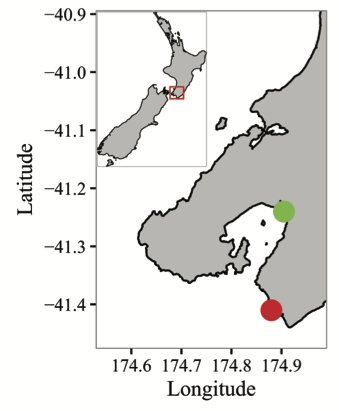
\includegraphics{images/nz_map.png}
\caption{\label{fig:nzmap}Sampling locations for juvenile G. maculatus.
Green = Hutt River. Red = Wainuiomata River. River mouths are
approximately 20 km apart. Data for the maps comes from the `maps'
(Becker et al. 2016) and `mapdata' (Becker et al. 2016) R packages.}
\end{figure}

\subsection{Statistical Analysis}\label{statistical-analysis}

To evaluate spatio-temporal variation in G. maculatus developmental
characteristics I fit three nested linear models (using standard length,
average growth rate, and age as response variables in three separate
models). Predictor variables included in each model were \emph{site}
(Hutt and Wainuiomata), \emph{month} (4 months in the Hutt, 3 in the
Wainuiomata), and \emph{day} (4 days per month for each site). I
included main effects of site, month, and day, and the interaction term
of site x month. The day effect was nested within the interaction term
as I only wanted to compare days that occurred within the same month and
site. I hypothesized that all three response variables would show
different patterns across months given divergent dispersal patterns and
associated environmental conditions experienced. I did not expect to see
any differences across days or between sites as I assumed larvae would
all have experienced similar environmental conditions (or similar enough
that differences would not be detectable). Therefore, I treated all
terms in the model as fixed effects so I could specifically evaluate the
differences between the levels of each factor. I conducted post hoc
tests, using the `lsmeans' procedure from the `lsmeans' package (Lenth
2016), to evaluate 4 aspects of each model: Do developmental
characteristics (1) vary between sites (main effect: site); and (2) vary
across months (main effect: month). (3) Does the pattern of variation
between sites differ across months (interaction: month x site). (4)
Using the nested term I also evaluated variation in developmental
characteristics across days within sites and months (nested main effect:
day). When there was a significant interaction, I ran post hoc tests to
evaluate aspects (1) and (2), see above. If there was no significant
interaction, post hoc tests were run on each main effect.

\section{Results}\label{results}

I evaluated spatial and temporal variation in developmental
characteristics with a sample of 496 fish. Standard length ranged from
33.7 to 51.2mm (mean = 45.5, SD = 2.3). Ages ranged from 105 to 233 days
(mean = 175, SD = 18.5). Otolith growth rates ranged from 1.27 to 2.25
μm-1day-1 (mean = 1.67, SD = 0.163).

\subsection{Spatio-temporal variation in standard
length}\label{spatio-temporal-variation-in-standard-length}

I found a non-significant effect of the interaction term (F2, 470 =
1.95, p = 0.144, \ref{fig:anova1}) suggesting that patterns of variation
in length across months were similar between sites. Therefore I
evaluated main effects. Fish from the Wainuiomata River were longer than
fish from the Hutt River (main effect of site variable, F1, 470 = 10.74,
p = 0.001, \ref{fig:stdlengthsite}).

\begin{figure}
\centering
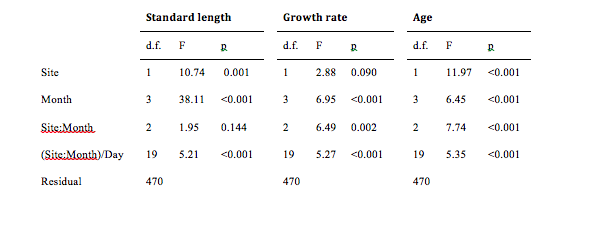
\includegraphics{images/anova_table1.png}
\caption{\label{fig:anova1}Spatio-temporal variation in length, growth rate,
and age of juvenile G. maculatus. ``Site:Month'' represents the
interaction term, and ``(Site:Month)/Day'' represents the day term,
nested within the month and site interaction term.}
\end{figure}

\begin{figure}
\centering
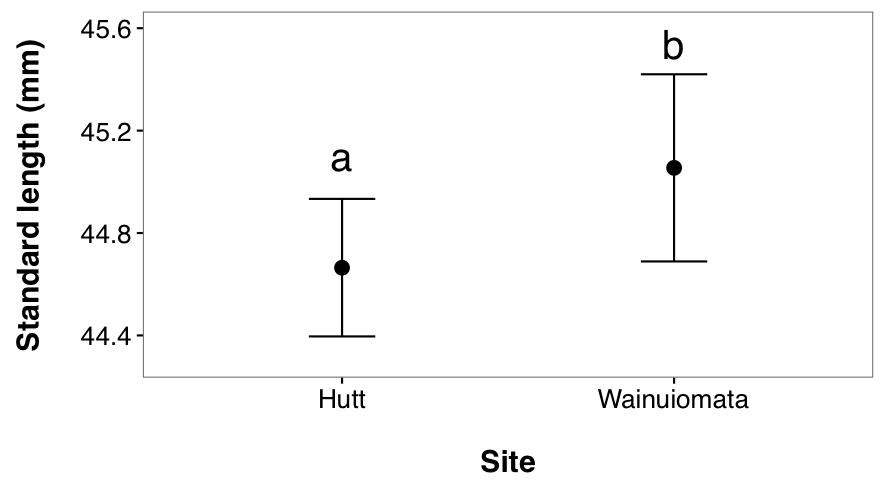
\includegraphics{images/std_length_fig1.png}
\caption{\label{fig:stdlengthsite}Spatial variation in standard length of
juvenile G. maculatus collected from two sites (Hutt River and
Wainuiomata River). Given are L-S means (i.e.~corrected for other
sources of variation in the statistical model, see table 2-1) ± 95\% CI.
Dissimilar lowercase letters indicate a significant difference based
upon post hoc tests.}
\end{figure}

Length also varied across months (main effect of month variable, F3, 470
= 38.11, p \textless{} 0.001, \ref{fig:stdlengthmonth}). A post hoc test
revealed that fish caught in August were significantly larger than fish
from September (p \textless{} 0.0001), October (p = 0.0026), and
November (p \textless{} 0.0001). Fish from September and October were
both significantly larger than November fish (p \textless{} 0.0001 for
both) but not different from one another (p = 0.4505).

\begin{figure}
\centering
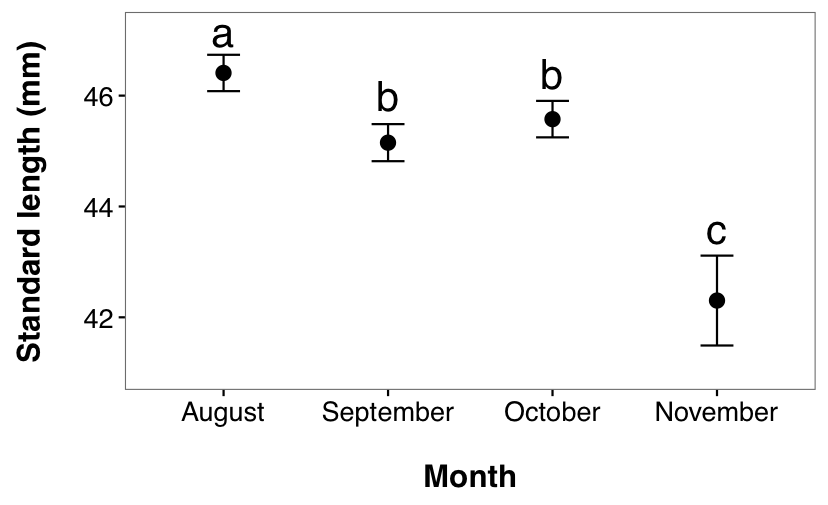
\includegraphics{images/stdlengthmonth.png}
\caption{\label{fig:stdlengthmonth}Temporal variation in standard length of
juvenile G. maculatus collected from two sites. Given are LS means ±
95\% CI. Dissimilar lowercase letters indicate a significant difference
based upon post hoc tests.}
\end{figure}

The standard length of G. maculatus varied significantly among days
nested within sites (F19, 470 = 5.210, p \textless{} 0.0001,
\ref{fig:spatiotemp1}). A post hoc test (\ref{fig:spatiotemp1table})
indicates that a small number of pairwise comparisons appear to be
driving the significance of this effect. \ref{fig:spatiotemp1} suggests
that sizes of G. maculatus are heterogeneous across consecutive days
within some months (i.e.~October, November) for the Hutt River in
particular.

\begin{figure}
\centering
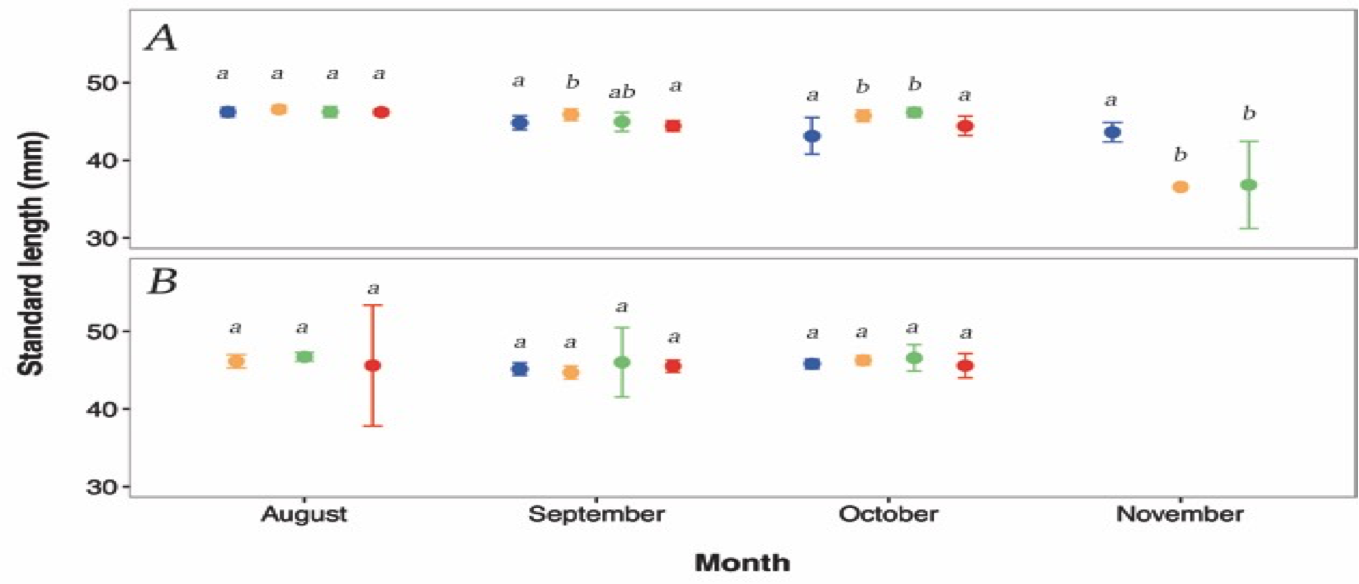
\includegraphics{images/spatiotemp1.png}
\caption{\label{fig:spatiotemp1}Daily (within month) temporal variation in
standard length between (A) Hutt River, and (B) Wainuiomata River. Given
are LS means ± 95\% CI. Different colours represent the different
sampling days. Blue=day 1, orange=day 2, green=day 3, red=day 4. Missing
symbols indicate days were no fish were sampled. Confidence intervals
are obscured by size of symbols for several observations. Dissimilar
lowercase letters indicate a significant difference based upon post hoc
tests; separate analyses were conducted for each site and month}
\end{figure}

\begin{figure}
\centering
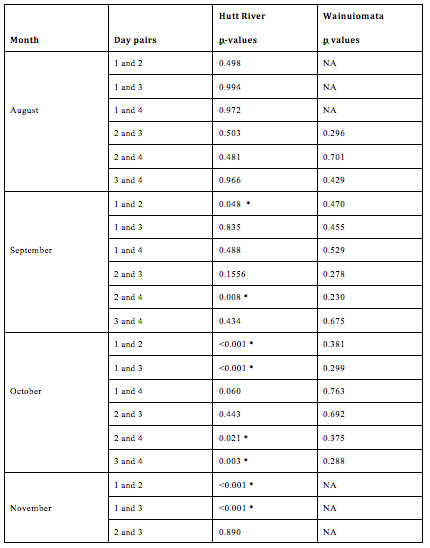
\includegraphics{images/spatiotemp1table.png}
\caption{\label{fig:spatiotemp1table}Pairwise comparisons of standard length
between days nested within months and sites. No fishing was conducted in
the Wainuiomata during November due to river mouth closure. No fish were
successfully caught on the 1st day in August in the Wainuiomata or the
4th day in November in the Hutt (as indicated by ``NA''). Asterisks
indicate a significant difference in length between day pairs.}
\end{figure}

\subsection{Spatio-temporal Variation in Average Growth
Rate}\label{spatio-temporal-variation-in-average-growth-rate}

I found a significant interaction between month and site (F2, 470 =
6.489, p = 0.0017, \ref{fig:spatiotemporalgrowthrate}), indicating that
growth rate changes over time and sites (\ref{fig:anova1}). A post hoc
test showed that, in the Hutt River, fish caught in August grew faster
than fish caught in September (p \textless{} 0.0001), October (p =
0.0265) and November (p = 0.0134). September did not differ to October
(p = 0.3105) or November (p \textgreater{} 0.9999). October and November
also did not differ (p = 0.6749). In the Wainuiomata River, August fish
did not have a significantly different growth rate to fish caught in
September (p \textgreater{} 0.9999) or October (p = 0.3072). Fish from
September and October also did not differ significantly (p = 0.5708).

\begin{figure}
\centering
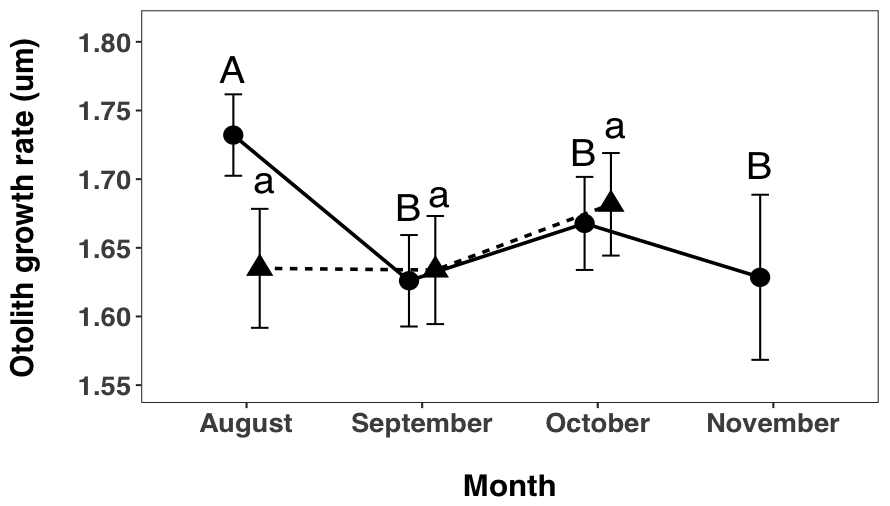
\includegraphics{images/spatiotemporalgrowthrate.png}
\caption{\label{fig:spatiotemporalgrowthrate}Spatial and temporal variation
in otolith growth rate of juvenile G. maculatus collected from two sites
(circles/uppercase letters: Hutt River, triangles/lowercase letters:
Wainuiomata River). Given are LS-means (i.e.~corrected for other sources
of variation in the statistical model (Table 2-1) ± 95\% CI. Dissimilar
letters indicate a significant difference within sites, across time
(e.g., no difference across months within the Wainuiomata River).
Sampling did not occur in the Wainuiomata River during November due to
river mouth closure.}
\end{figure}

The otolith growth rate varied significantly among days nested within
months and sites (F19, 470 = 5.2703, p \textless{} 0.0001,
\ref{fig:growthratebyday}). A post hoc test (Table 2 3) indicates that a
small number of pairwise comparisons are driving the significance of
this effect. \ref{fig:growthratebyday} suggests that otolith growth
rates of G. maculatus are heterogeneous across days within all months
for the Hutt River and homogenous across days within all months for the
Wainuiomata River.

\begin{figure}
\centering
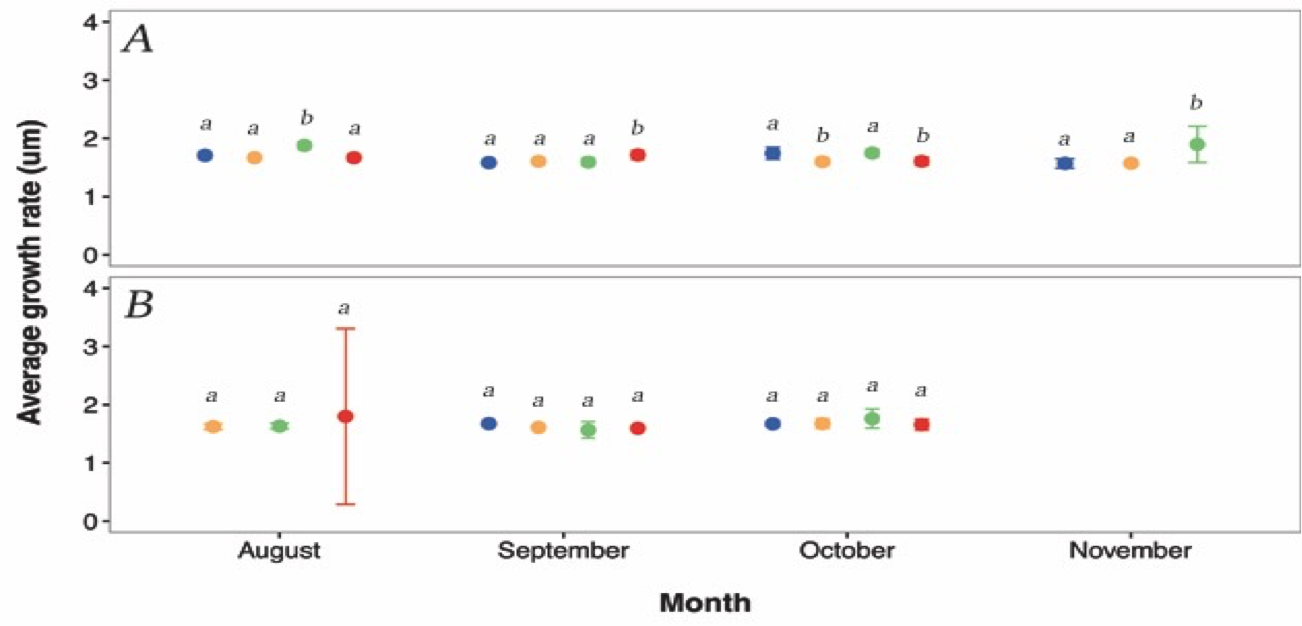
\includegraphics{images/growthratebyday.png}
\caption{\label{fig:growthratebyday}The otolith growth rate varied
significantly among days nested within months and sites (F19, 470 =
5.2703, p \textless{} 0.0001, Figure 2 6). A post hoc test (Table 2 3)
indicates that a small number of pairwise comparisons are driving the
significance of this effect. Figure 2 6 suggests that otolith growth
rates of G. maculatus are heterogeneous across days within all months
for the Hutt River and homogenous across days within all months for the
Wainuiomata River.}
\end{figure}

\begin{figure}
\centering
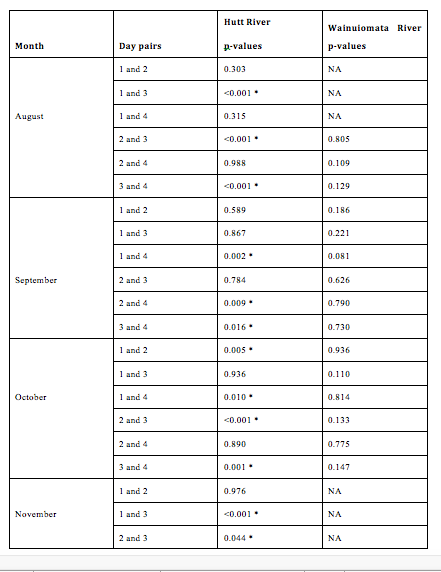
\includegraphics{images/spatiotemp2table.png}
\caption{\label{fig:spatiotemptable2}Pairwise comparisons of average otolith
growth rate between days nested within months and sites. No fishing was
conducted in the Wainuiomata during November due to river mouth closure.
No fish were successfully caught on the 1st day in August in the
Wainuiomata or the 4th day in November in the Hutt (as indicated by
``NA''). Asterisks indicate a significant difference in length between
day pairs.}
\end{figure}

\subsection{Spatio-temporal Variation in
Ages}\label{spatio-temporal-variation-in-ages}

I found a significant interaction between month and site (F2, 470 =
7.7421, p = 0.0004, \ref{fig:spatiotemporalage}), indicating that
patterns of age variation changed across time and sites. A post hoc test
showed that, in the Hutt River, fish caught in August were significantly
younger than fish caught in September (p \textless{} 0.0001), and
October (p = 0.0029) but not November (p = 0.3783). Fish caught in
September did not differ to fish from October (p = 0.4134) or November
(p = 0.2774). There was also no difference in fish caught from October
and November (p = 0.8869). In the Wainuiomata River, fish caught in
August showed no difference in age to fish caught in September (p =
0.9934) or October (p = 0.7513). Fish caught in September also showed no
difference to fish caught in October (p = 0.8709).

\begin{figure}
\centering
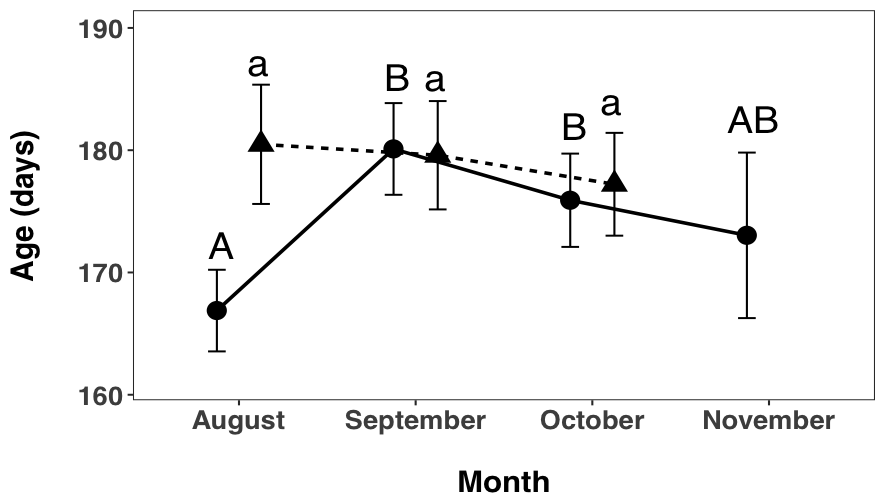
\includegraphics{images/spatiotemporalage.png}
\caption{\label{fig:spatiotemporalage}I found a significant interaction
between month and site (F2, 470 = 7.7421, p = 0.0004, Figure 2 7),
indicating that patterns of age variation changed across time and sites.
A post hoc test showed that, in the Hutt River, fish caught in August
were significantly younger than fish caught in September (p \textless{}
0.0001), and October (p = 0.0029) but not November (p = 0.3783). Fish
caught in September did not differ to fish from October (p = 0.4134) or
November (p = 0.2774). There was also no difference in fish caught from
October and November (p = 0.8869). In the Wainuiomata River, fish caught
in August showed no difference in age to fish caught in September (p =
0.9934) or October (p = 0.7513). Fish caught in September also showed no
difference to fish caught in October (p = 0.8709).}
\end{figure}

The ages of juvenile G. maculatus differed significantly among days
nested within month and site (F19, 470 = 5.3537, p \textless{} 0.0001,
\ref{fig:spatiotemp3}). A post hoc test (\ref{fig:spatiotemp3table})
again indicates that the significance of this effect is driven by a
small number of pairwise comparisons in the Hutt River.
\ref{fig:spatiotemp3} suggests that ages of G. maculatus are
heterogeneous across days within all months for the Hutt River and
homogenous across days within all months for the Wainuiomata River.

\begin{figure}
\centering
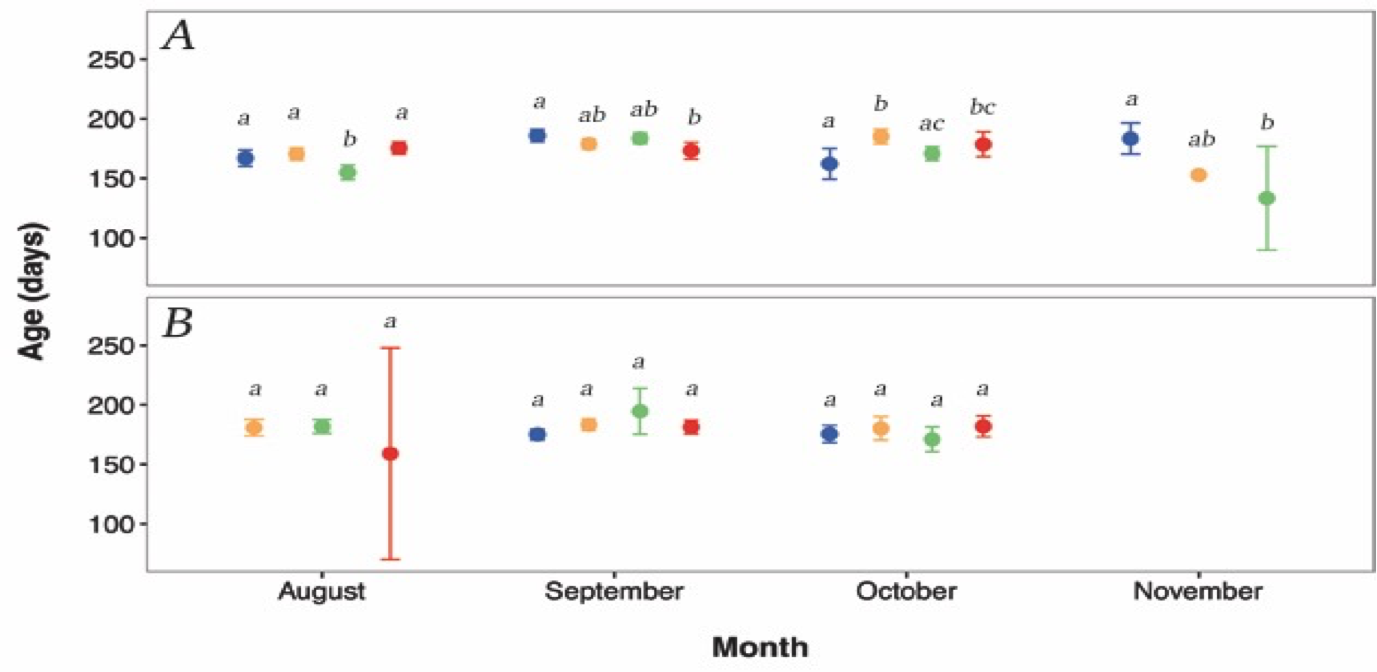
\includegraphics{images/spatiotemp3.png}
\caption{\label{fig:spatiotemp3}Daily (within month) temporal variation in
age between (A) Hutt River, and (B) Wainuiomata River. Different colours
represent the different sampling days. Blue=day 1, orange=day 2,
green=day 3, red=day 4. Missing symbols indicate days were no fish were
sampled. Error bars represent 95\% confidence intervals. Confidence
intervals are obscured by size of symbols for several observations.
Dissimilar lowercase letters indicate a significant difference based
upon post hoc tests; separate analyses were conducted for each site and
month. Sampling did not occur in the Wainuiomata River during November
due to river mouth closure.}
\end{figure}

\section{Discussion}\label{discussion}

\subsection{Summary of Results}\label{summary-of-results}

I found site-specific trends in the developmental histories of G.
maculatus. Juvenile G. maculatus entering the Wainuiomata River showed
no difference in growth rate or age across months, although they did
show a decrease in standard length across months. Fish from the Hutt
River also shared this decrease in standard length, but also showed a
decrease in otolith growth rate. Age showed a hump shaped curve, where
the youngest recruiting fish were in August and November. Fish in the
Hutt River during August, were the youngest, fastest growing, and
largest, a pattern that was not reflected in the Wainuiomata. However,
while fish from the Wainuiomata River did not show significant
differences in otolith growth rate and age, there did appear to be
non-significant trends that matched the results from the Hutt River.

There was no day-to-day variation in any developmental characteristics
of fish sampled from the Wainuiomata River. While fish from the Hutt
River did show day-to-day variation, there was significant variation in
the direction and magnitude of trends. Therefore, the two main points of
interest become (1) why was there daily and monthly variation through
time, and (2) why was there more variation in the Hutt River?

\subsection{Spatial Differences in Developmental
Histories}\label{spatial-differences-in-developmental-histories}

I propose two hypotheses that could explain my results (and these are
not mutually exlusive): (1) the Hutt River may be replenished by fish
from a wider variety of source populations than the Wainuiomata River,
which could lead to greater variation in developmental histories among
cohorts (natal source hypothesis), and/or (2) recruits from the Hutt
River may have experienced greater environmental variability during
their pelagic larval dispersal phase, which could lead to different
phenotypic distributions through individual fish experiencing phenotypic
plasticity or selective mortality (environmental experience hypothesis).

A difference in the composition of source populations entering each
river is dependent on the extent of dispersal. G. maculatus have very
strong swimming capabilities (Barker and Lambert 1988), and considerable
research has examined the extent of population mixing and natal return
(Barker and Lambert 1988, Berra et al. 1996, Waters and Burridge 1999,
Waters et al. 2000) with current paradigms suggesting that G. maculatus
does not show extensive natal homing (Waters et al. 2000, Hickford and
Schiel 2016). However most evidence is based off a lack of genetic
structure among sampled populations, and genetic structuring may be
mediated by only a small number of mixing individuals (Hartl 1988).
Furthermore, most studies have been concerned with broad spatial
hypotheses (Barriga et al. 2007, Barbee et al. 2011, Barriga et al.
2012), rather than considering the characteristics of individual systems
that may facilitate a higher level of retention than the majority of
source populations. Harbour systems have been shown to have highly
retentive properties due to physical and hydrodynamic processes acting
on the water currents (Maxwell 1956, Bowman et al. 1983, Anderson 1988).
Therefore I suggest that the hydrodynamic characteristics of the
Wellington Harbour may promote higher retention of larval G. maculatus
than would be expected by a coastally positioned system, thus promoting
self recruitment (Jones et al. 2005, Levin 2006, McDowall 2009).
However, I do not assume that the Wellington Harbour is completely
isolated from other (perhaps coastally derived) G. maculatus
populations, and I would expect it to still receive input from other
source populations around New Zealand (McDowall et al. 1975, Caley et
al. 1996, McDowall 2002, Swearer et al. 2002). The combined input of
recruits from other source populations (with their own variations in
phenotype), plus the resident population in the Wellington Harbour, may
combine to produce a more heterogeneous population of G. maculatus
(Shima and Swearer 2009). Fish from the Wellington Harbour would
therefore show a wider distribution in phenotypes than the Wainuiomata
River, which may not have a resident population, and is only replenished
by regional source populations (that shared more similar environmental
conditions). These differences in the spread of potential phenotypes may
be driving the lack of significant differences in the Wainuiomata, while
accounting for the range of patterns documented in the Hutt River.

Marine habitats can show considerable variation in temperature, water
flow, light availability, and salinity (Johnston 2006) which may vary
extensively through time. Pelagic fish may experience phenotypic
plasticity as a result of this environmental variability, and therefore
their phenotype may correlate with conditions experienced during
dispersal. If my two study sites are replenished by different
combinations of source populations, with differing dispersal histories,
then the environmental conditions experienced may be driving these site
specific differences. During dispersal, cohorts may encounter novel
environments that impose directional selection on phenotypic traits
(Reznick and Ghalambor 2001, Grether 2005), which shifts the mean
phenotype to a new peak (Lande and Arnold 1983). Environmental pressures
may be either biotic (Handelsman et al. 2013) or abiotic (Carrera et al.
2012) but all have the potential to drive phenotypic shifts (Agrawal
2001). This hypothesis is dependent upon Wellington Harbour showing a
higher degree of temporal variability in its biotic and abiotic
conditions. Under the assumption that it is more variable, individuals
with recent resident periods in the harbour may have experienced
phenotypic plasticity, and therefore developed phenotypic
characteristics representative of the conditions at the time (Agrawal
2001, Barriga et al. 2012, Chapman et al. 2015). Depending on the scale
of this variability it may account for both monthly and daily
differences. In contrast, if the Cook Strait shows a less temporally
variable environment then that may explain the fairly consistent trends
in phenotypes of recruits.

General trends in harbour systems have shown evidence of circulation
currents leading to high levels of nutrients (Mackas and Harrison 1997)
and zooplankton (Soetaert and Herman 1994). They have also shown that
abiotic conditions can be highly variable between seasons (Muylaert and
Raine 1999). Results by Maxwell (1956) indicate average water
temperatures in the Wellington Harbour increase from August to November,
yet there is also considerable fluctuation over shorter time scales,
with changes of up to 2.5°C within a three day period. Maxwell (1956)
also postulated that the causes of this high variability was due to the
sheltered positioning of the harbour. In contrast, Cook Strait has very
high energy, fast flowing currents (Bowman et al. 1983), and its lack of
shelter may not promote high levels of abiotic variability. Cook Strait
is highly dynamic with complex patterns of water circulation, but there
is little evidence for its low productivity waters being temporally
variable (Bowman et al 1983). While it may be a high energy environment,
I argue that the consistent nature of it is not enough to drive
phenotypic differences in resident cohorts of G. maculatus.

\chapter{Applications}\label{applications}

Some \emph{significant} applications are demonstrated in this chapter.

\section{Example one}\label{example-one}

\section{Example two}\label{example-two}

\chapter{Final Words}\label{final-words}

We have finished a nice book.

\bibliography{book.bib,packages.bib}

\end{document}
